\documentclass[tikz]{standalone}
\usepackage{tikz}
\usepackage{alphalph}
\usetikzlibrary{positioning, graphs}
\usetikzlibrary{graphs.standard}
\begin{document}
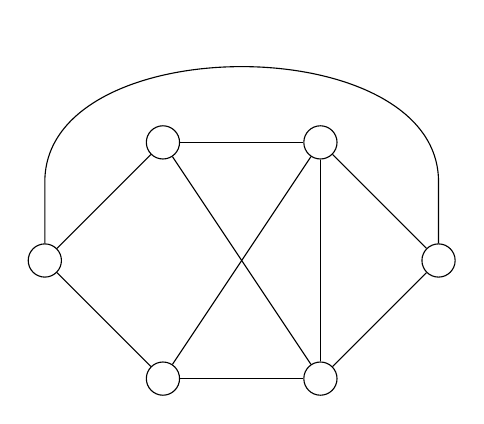
\begin{tikzpicture}
\begin{scope}
		[vertex/.style={draw,circle,inner sep = 0em, minimum size = 1.2em},
		 edgelabel/.style = {fill = white, inner sep = 0.2em, font=\small}]
		\node[vertex] (s) at (0.5, 0) {};
		\node[vertex] (a) at (2,  1.5) {};
		\node[vertex] (b) at (4,  1.5) {};
		\node[vertex] (c) at (2, -1.5) {};
		\node[vertex] (d) at (4, -1.5) {};
		\node[vertex] (t) at (5.5, 0) {};
		
        \draw[-] (s) to (a);
        \draw[-] (s) to (c);
        \draw[-] (a) to (b);
        \draw[-] (a) to (d);
        \draw[-] (b) to (c);
        \draw[-] (b) to (d);
        \draw[-] (b) to (t);
        \draw[-] (c) to (d);
        \draw[-] (d) to (t);
        \draw[-, out=90, in=90] (s) -- ++(0, 1) to ++(5, 0) -- (t);
		
\end{scope}
\end{tikzpicture}
\end{document}